\section{Data Randomization Test}

\begin{figure*}
    \centering
    \begin{subfigure}{\textwidth}
        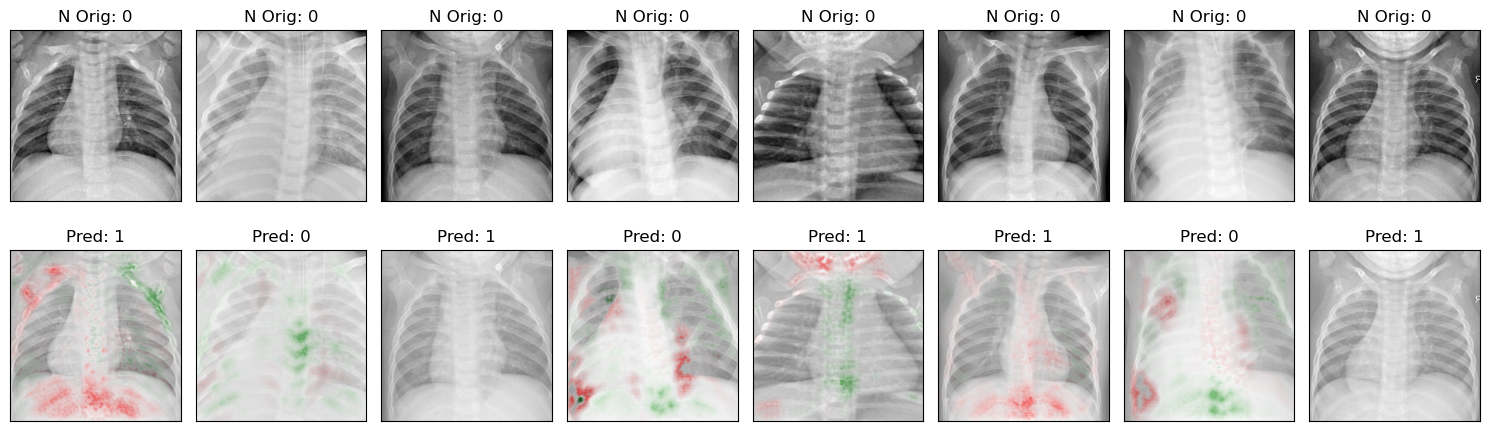
\includegraphics[width=1\textwidth]{images/ig_rand_train.png}
    \end{subfigure}
    \centering
    \begin{subfigure}{\textwidth}
        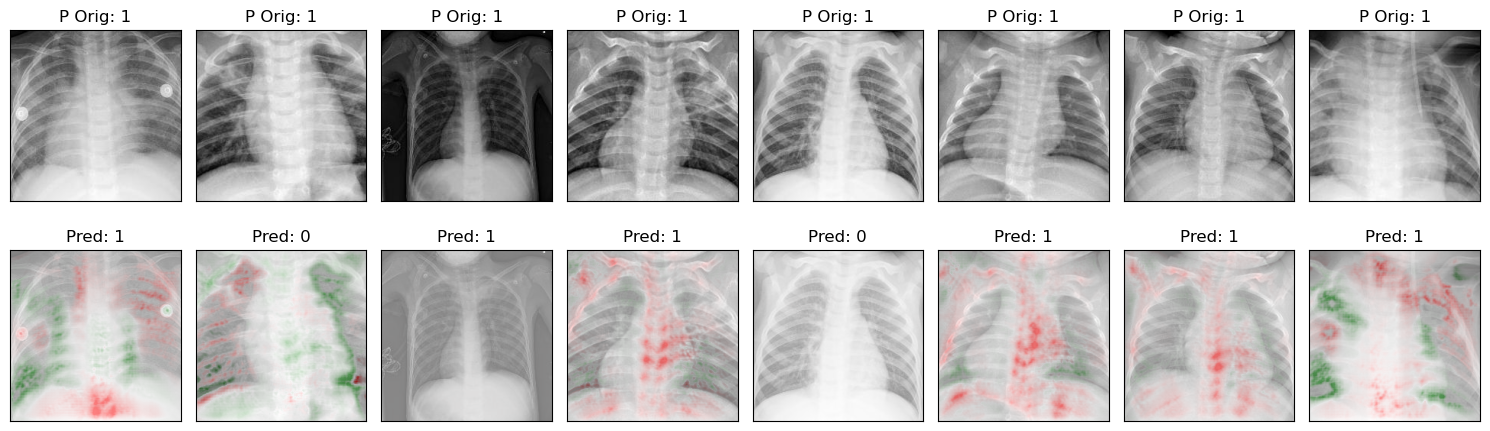
\includegraphics[width=1\textwidth]{images/ig_rand_train_P.png}
    \end{subfigure}
    \caption{Training images to which integrated gradients was applied. The model was finetuned on random labels. Upper two rows are from healthy patients, bottom two rows from patients with pneumonia. The 1st and 3rd row contain the input image, the 2nd and 4th row contain an added overlay from integrated gradients. In red is the negative attribution, in green the positive attribution.}
    \label{fig:ig_rand_train}
\end{figure*}

For the data randomization test, we train our model with random labels to ensure it isn't just a fancy edge detector.

We tried two approaches. First, we tried to train a model from scratch, with the same settings and parameters as before, but with randomized labels. We trained for many epochs (50 in total), but at no point was the model able to learn something useful, and applying Grad-CAM or integrated gradients only resulted in an empty overlay. This of course meant that our initial model was able to learn relevant information from the X-ray images.

Still, to allow for better visualization, we tried a second approach: we fine-tuned our model for 16 epochs on random labels, after pre-training on the true labels for 7 epochs. The fine-tuning was stopped when the variance of the predicted results was near 0, which coincided with the end of epoch 16. This was to ensure that the model was not too confident in its predictions.
The accuracy on the test set was, as expected, around 50\%. Precision and recall also had values close to 0.5.

\subsection*{A. Integrated Gradients}

For integrated gradients, there seems to be an increased focus on bone tissue, similar to what we observed when training on true labels, but this time, it is likely due to the sensitivity of the model to white areas. For example, in Figure \ref{fig:ig_rand_train} some images highlight the ribs itself instead of the area of lung tissue in between. In addition, the border of the heart is marked more clearly than before.

\begin{figure}
    \centering
    \begin{subfigure}{\columnwidth}
        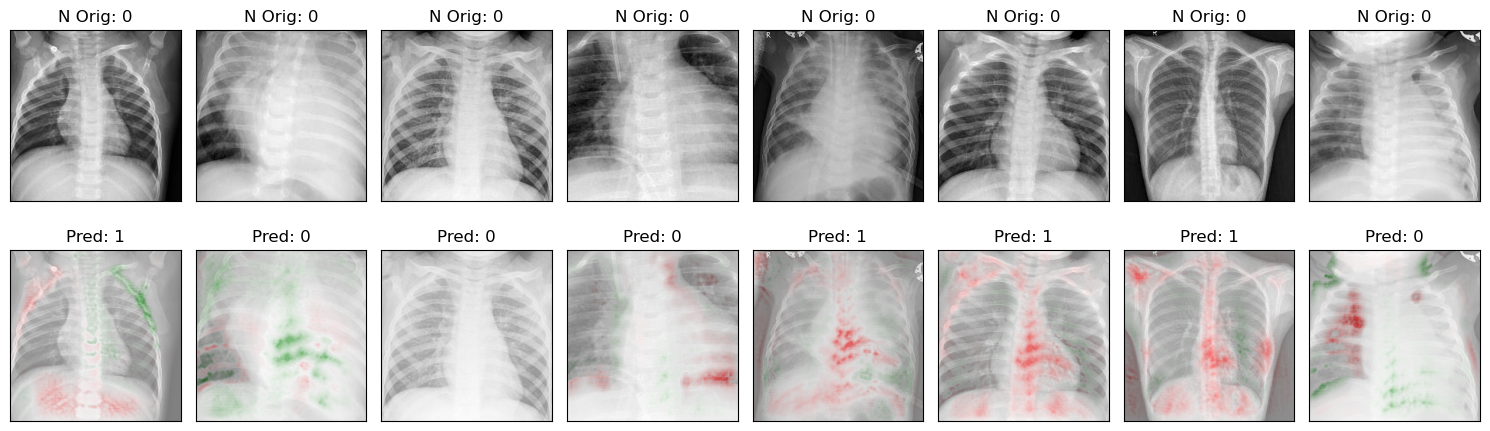
\includegraphics[width=1\textwidth]{images/ig_rand_test.png}
    \end{subfigure}
    \centering
    \begin{subfigure}{\columnwidth}
        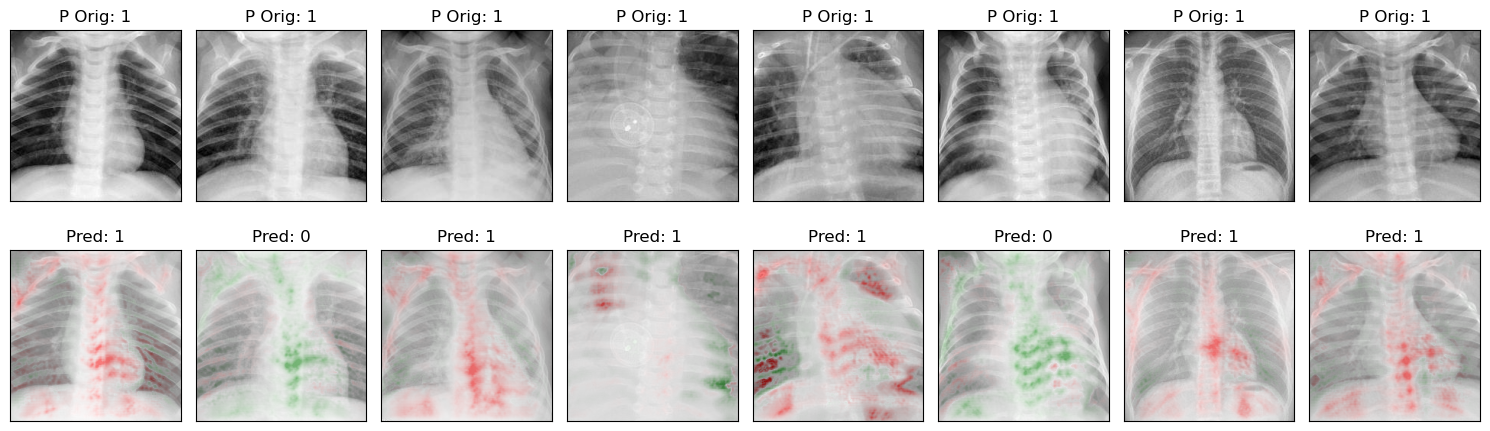
\includegraphics[width=1\textwidth]{images/ig_rand_test_P.png}
    \end{subfigure}
    \caption{Test images to which integrated gradients was applied. The model was finetuned on random labels. Upper two rows are from healthy patients, bottom two rows from patients with pneumonia. The 1st and 3rd row contain the input image, the 2nd and 4th row contain an added overlay from integrated gradients. In red is the negative attribution, in green the positive attribution.}
    \label{fig:ig_rand_test}
\end{figure}

Another interesting feature is how much focus the model puts on the diaphragm, which is more opaque when compared to lung tissue.

There does not seem to be a clear difference between features of patients labeled as healthy or sick (and the model predicts most patients as sick anyway).

In conclusion, it seems that the model fine-tuned on random labels simply looks at brighter areas, i.e. dense tissues such as bone. This shows that our initial 'true' model did in fact learn to correctly attribute certain areas of the X-ray to certain classes.

The same trends can be seen for the test data in Figure \ref{fig:ig_rand_test}.


\subsection*{B. Grad-CAM}

Note that instead of clipping the overlay at 0, like in Q4 (normal ReLU), we clip the values of the localization map at -0.5. The reason for this being that clipping at 0 simply gave a purple screen (0 values everywhere), due to the lack of attribution obtained from the model. In the paper, the authors mention that without ReLU, the localization maps sometimes highlight more than just the desired class and perform worse at localization. Still, since we only have two classes and would like to properly explain at least something, we opt to clip at -0.5.

In Figure \ref{fig:gc_rand_train}, observations are consistent with each other and between both classes. We can see an outline of the two lungs and the empty space surrounding the patients in all images in purple/blue/azure, showing that the model was mainly focusing on darker intensities (since we only look at negative values), agreeing with the green/yellow color.

\begin{figure*}
    \centering
    \begin{subfigure}{\textwidth}
        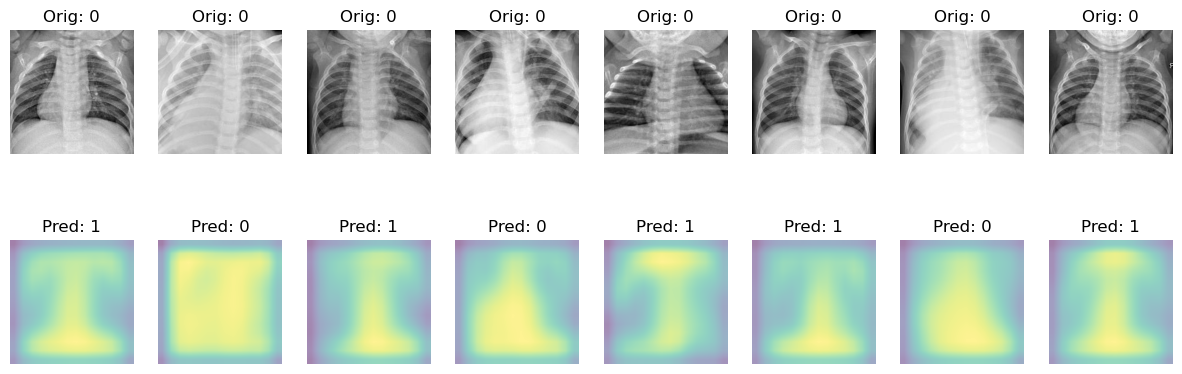
\includegraphics[width=1\textwidth]{images/gc_rand_train.png}
    \end{subfigure}
    \centering
    \begin{subfigure}{\textwidth}
        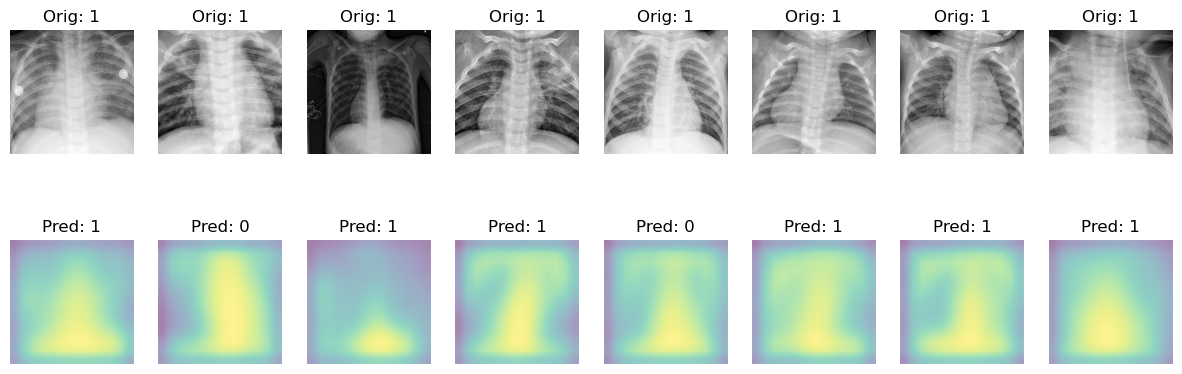
\includegraphics[width=1\textwidth]{images/gc_rand_train_P.png}
    \end{subfigure}
    \caption{Training images to which Grad-CAM was applied. The model was finetuned on random labels. Upper two rows are from healthy patients, bottom two rows from patients with pneumonia. The 1st and 3rd row contain the input image, the 2nd and 4th row contain the overlay produced by Grad-CAM. Yellow signifies the highest attribution, purple the lowest attribution.}
    \label{fig:gc_rand_train}
\end{figure*}

\begin{figure}
    \centering
    \begin{subfigure}{\columnwidth}
        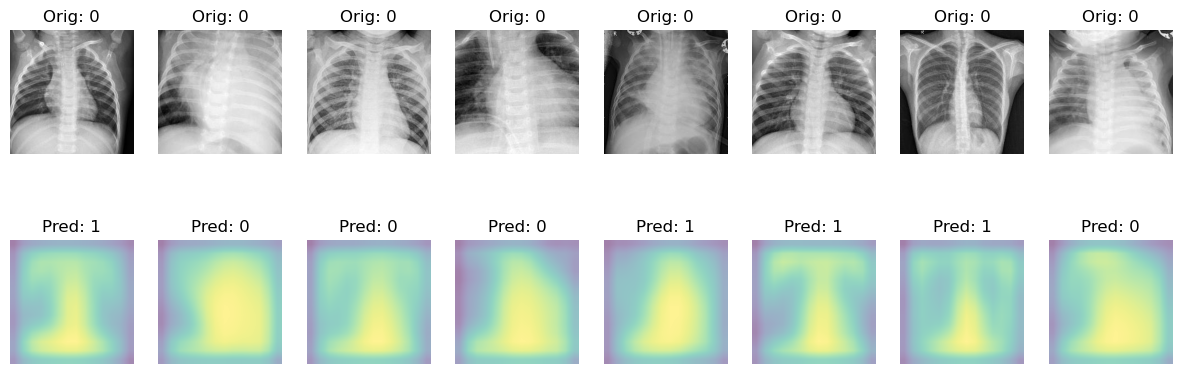
\includegraphics[width=1\textwidth]{images/gc_rand_test.png}
    \end{subfigure}
    \centering
    \begin{subfigure}{\columnwidth}
        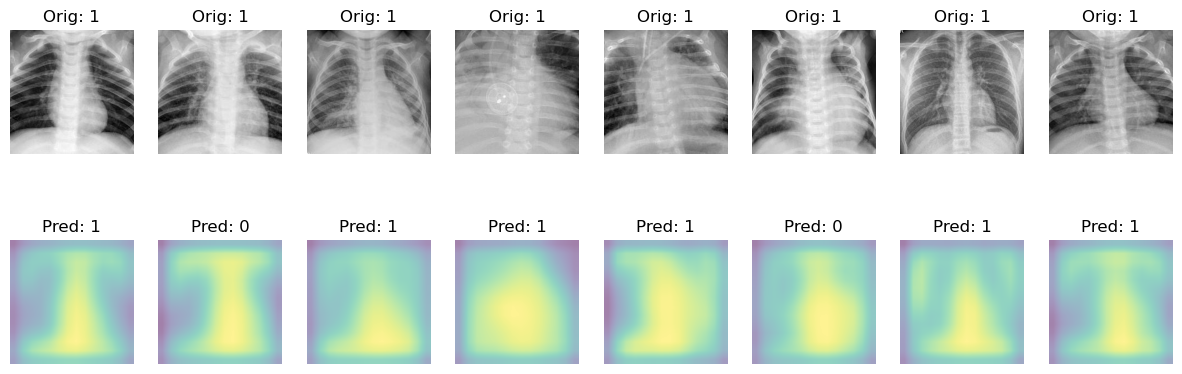
\includegraphics[width=1\textwidth]{images/gc_rand_test_P.png}
    \end{subfigure}
    \caption{Test images to which Grad-CAM was applied. The model was finetuned on random labels. Upper two rows are from healthy patients, bottom two rows from patients with pneumonia. The 1st and 3rd row contain the input image, the 2nd and 4th row contain the overlay produced by Grad-CAM. Yellow signifies the highest attribution, purple the lowest attribution.}
    \label{fig:gc_rand_test}
\end{figure}


Visualization of the test set in Figure \ref{fig:gc_rand_test} confirms the previously mentioned observations.